\documentclass[conference]{IEEEtran}

\usepackage{mathptmx} % Times Roman Font

\usepackage{helvet} % Arial/Helvetica font
\renewcommand{\familydefault}{\sfdefault} % Makes serif text all Helvetica

\usepackage[left=0.5cm, right=0.5cm, top=0.5cm]{geometry} % Sets the page margins

\usepackage{graphicx}

\usepackage{multicol}
\usepackage{float}

\usepackage{caption}

\captionsetup[table]{skip=10pt} % Adjusts space between table and caption

\usepackage{ragged2e}

\usepackage{array}
\newcolumntype{L}[1]{>{\raggedright\arraybackslash}p{#1}}

\title{Case Study 3: ECG Analysis}
\date{}

\begin{document}
\justifying

\maketitle

\section{Introduction} 

This document aims to provide an analysis of observations taken from an electrocardiogram (ECG). ECG is a technique for recording the electrical activity of a patients heart over time. It can provide details about the heart's rate and rhythm.

An ECG waveform consists of a P wave, QRS complex, and T wave. These distinctive characteristics correspond to different stages of the heart's electrical cycle. The R wave (of the QRS complex) is the most prominent feature and can be assessed to measure RR intervals (the peak-peak time between R waves) and heart rate. Heart rates below 60 BPM are known as bradycardia and heart rates above 100 BPM are known as tachycardia. If an individual has a resting heart rate outside these parameters then it may be indicative of a heart complication.

The patient that the ECG data was collected from has been fitted with a pacemaker. The presence of a pacemaker can significantly alter the shape of the ECG waveform. Sharp spikes known as pacemaker spikes may appear, typically preceding the P wave or QRS complex depending on the type of pacing (atrial, ventricular, or dual-chamber).

\section{Observations and Justifications}

\subsection{Entire Waveform}

The ECG shows a complete lack of P waves throughout the entire waveform. While RR peak intervals appear consistent, the presence of a pacemaker is likely preventing the intervals from varying considerably. The lack of atrial activity suggests the patient has likely been diagnosed with atrial fibrillation and has hence been fitted with a pacemaker.

Table.~\ref{tab:times} shows the different rhythms throughout the recording. The patient has a consistent HR of approximately 70 BPM throughout with a small rise to approximately 78 BPM for approximately 3 minutes. This is not significant and can easily be caused by the patient moving slightly.

\subsection{Heart Rate}

By identifying all the R wave peaks above a set threshold, the RR intervals are measurable. We can then compute the distance between them to estimate the immediate heart rate (HR) at that point. By plotting the HR along the wave, we can highlight any obvious events. These events will appear as large positive or negative deflections as the distance between the R wave peaks will be increased or decreased depending on how the threshold R wave peak detection is calibrated. If a pacemaker spike is included as an R wave peak the HR will deflect positively. If the pacemaker spike is not included as an R wave peak the HR will deflect negatively. From Figure.~\ref{fig:HeartRate} we can calculate parameters of the patient's HR.

A mean heart rate of 72.76 and a standard deviation of 2.53 BPM were calculated and show that the rhythm is consistent for the measured waveform. Furthermore, 72.76 BPM is a healthy heart rate and within the bounds of bradycardia and tachycardia. 

\begin{figure}[h]
\centering
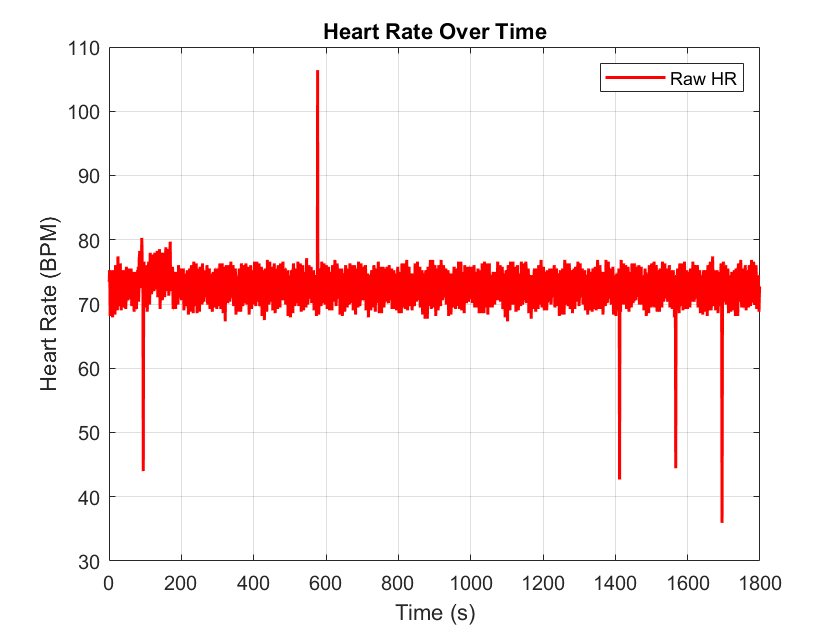
\includegraphics[width=10cm]{images/HR}
\caption{Graph to show the instant heart rate along the signal. Points where the RR interval is decreased will result in spikes where arrhythmia events are likely to have occurred.}
\label{fig:HeartRate}
\end{figure}

\subsection{Time Points of Normal Sinus Rhythm and Arrhythmia}

Five events were identified from Figure.~\ref{fig:HeartRate}. These events were assessed individually by locating the exact time point they occurred at and producing figures for each. Time points can be seen in Table.~\ref{tab:spikes}. 

\begin{table}[h]
\centering
\begin{tabular}{|c|c|c|}
\hline
\textbf{No.} & \textbf{Event} & \textbf{Time (s)} \\
\hline
1 & Pacemaker Spike & 95.15\\
2 & Pacing Artifact & 576.79 \\
3 & Pacemaker Spike & 1412.10\\
4 & Pacemaker Spike & 1567.34 \\
5 & ECG Artifact & 1567.34 \\

\hline
\end{tabular}
\caption{Time Points of Events}
\label{tab:spikes}
\end{table}



\begin{table}[h]
\centering
\begin{tabular}{|c|c|c|c|}
\hline
\textbf{Rhythm} & \textbf{Start Time (s)}  & \textbf{End Time (s)} & \textbf{Duration (s)} \\
\hline
Normal & 0 & 80 & 80\\
Elevated HR & 80 & 170 & 90\\
Normal & 170 & 1800 & 1630\\

\hline
\end{tabular}
\caption{Time Points and Durations of Rhythms}
\label{tab:times}
\end{table}

\subsection{Arrhythmia Events}

Events 1,3,4 can be seen in Figure.~\ref{fig:E1}, Figure.~\ref{fig:E3}, Figure.~\ref{fig:E4} respectively. The main features can be identified from them are a wide QRS complex (200-300ms) and a large negative spike before the QRS complex. These are consistent with pacemaker spikes.

From these features, We can predict that the patient is equipped with a pacemaker in ventricular pacing and sensing (VVI) mode. These are commonly fitted to patients with atrial fibrillation or flutter.

\begin{figure}[ht]
\centering
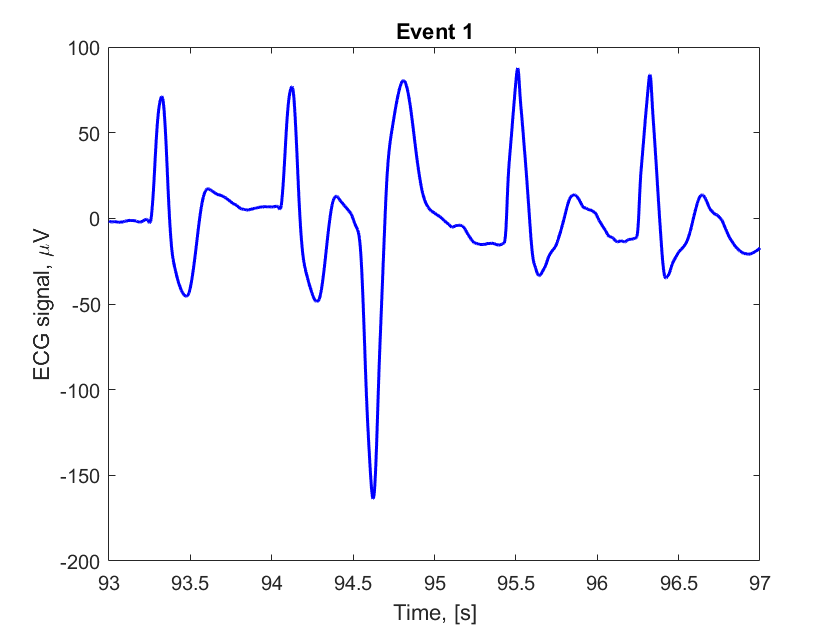
\includegraphics[width=10cm]{images/E1.png}
\caption{Graph to show Event 1. A large negative spike caused by the pacemaker followed by an extended QRS complex.}
\label{fig:E1}
\end{figure}

\begin{figure}[ht]
\centering
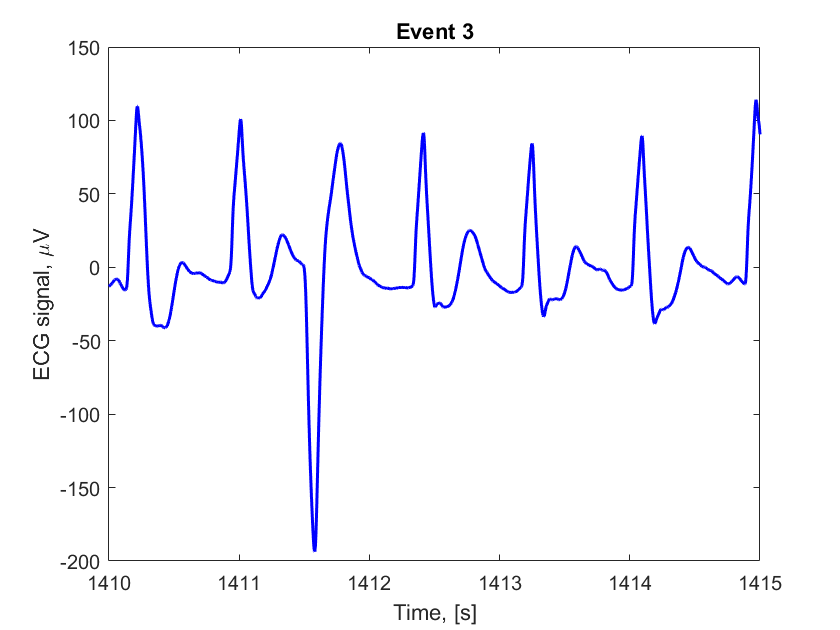
\includegraphics[width=10cm]{images/E3.png}
\caption{Graph to show event 3. A large negative spike caused by the pacemaker followed by an extended QRS complex.}
\label{fig:E3}
\end{figure}

\begin{figure}[ht]
\centering
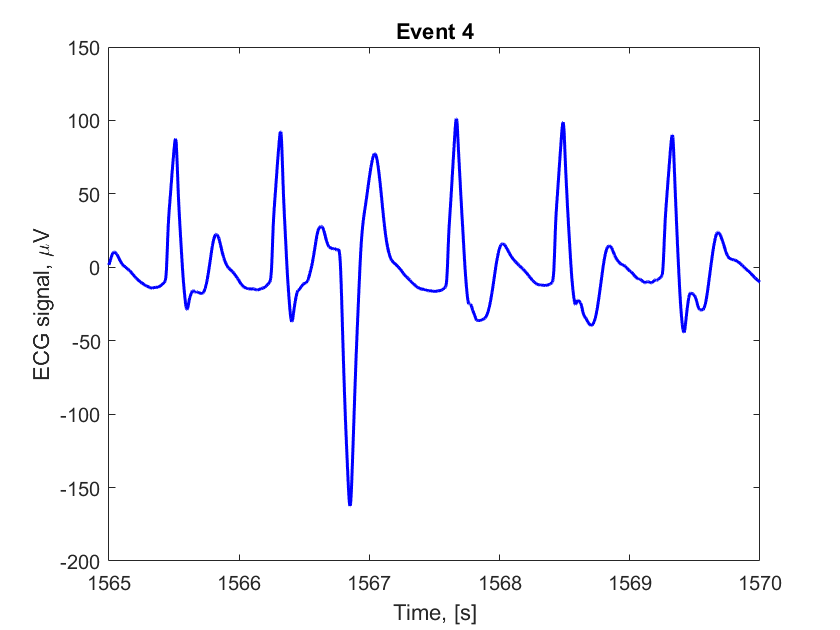
\includegraphics[width=10cm]{images/E4.png}
\caption{Graph to show Event 4. A large negative spike caused by the pacemaker followed by an extended QRS complex.}
\label{fig:E4}
\end{figure}

\subsection{Other Artifacts}
Event 2 can be seen in Figure.~\ref{fig:E2}. This appears to be a pacing artifact that causes a spike during the T wave, resulting in the T wave being split in two.

\begin{figure}[ht]
\centering
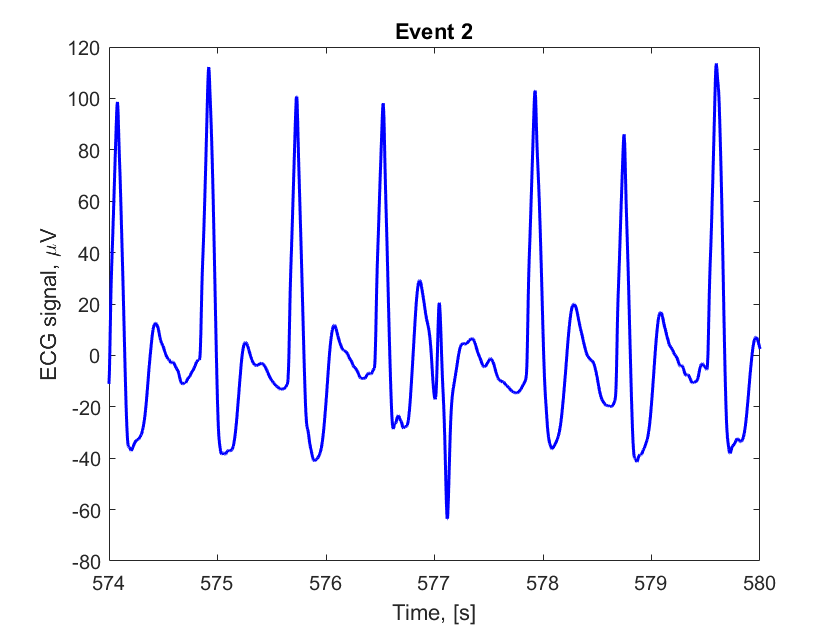
\includegraphics[width=10cm]{images/E2.png}
\caption{Graph to show event 2}
\label{fig:E2}
\end{figure}

Event 5 appears to have a regular rhythm but with a small decrease in the QRS complex amplitude. This can be assumed to be a random artefact with the ECG recording.

% \begin{figure}[ht]
% \centering
% 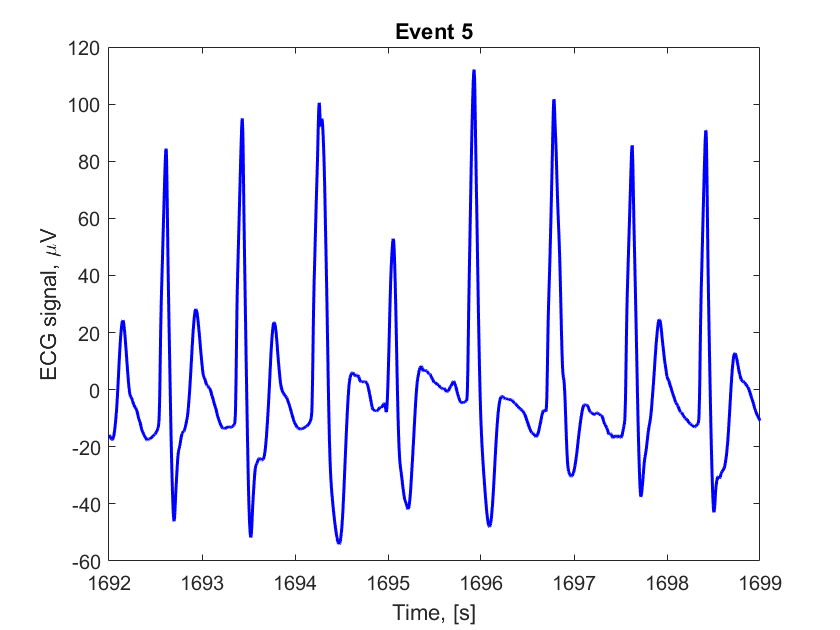
\includegraphics[width=10cm]{images/E5.png}
% \caption{Graph to show event 5}
% \label{fig:E5}
% \end{figure}



\section{Conclusion}

To conclude, four arrhythmia events were identified through high contrast variations in RR intervals. Each event's time point was identified and each was segmented and localised. We can assume that this patient is equipped with a pacemaker in VVI mode to assist with atrial fibrillation.
\bibliographystyle{IEEEtran}
% \bibliography{references} 
\end{document}